\documentclass{report}
\usepackage{graphicx, tikz-cd, float, titlepic, booktabs} % Required for inserting images
\usepackage{pgfplots}
\pgfplotsset{compat=1.15}
\usepackage{mathrsfs}
\usetikzlibrary{arrows}
\usepackage{amsmath, amssymb, amsthm, amsfonts, siunitx, physics, gensymb}
\AtBeginDocument{\RenewCommandCopy\qty\SI}
\usepackage[version=4]{mhchem}
\usepackage[most,many,breakable]{tcolorbox}
\usepackage{xcolor, fancyhdr, varwidth}
\usepackage[Glenn]{fncychap}
%Options: Sonny, Lenny, Glenn, Conny, Rejne, Bjarne, Bjornstrup
\usepackage{hyperref, cleveref}
\usepackage{icomma, enumitem} %comma as decimal and continue enumerate with [resume]
\usepackage[danish]{babel}
%%%%%%%%%%%%%%%%%%%%%%%%%%%%%%
% SELF MADE COLORS
%%%%%%%%%%%%%%%%%%%%%%%%%%%%%%
\definecolor{myg}{RGB}{56, 140, 70}
\definecolor{myb}{RGB}{45, 111, 177}
\definecolor{myr}{RGB}{199, 68, 64}
\definecolor{mytheorembg}{HTML}{F2F2F9}
\definecolor{mytheoremfr}{HTML}{00007B}
\definecolor{mylenmabg}{HTML}{FFFAF8}
\definecolor{mylenmafr}{HTML}{983b0f}
\definecolor{mypropbg}{HTML}{f2fbfc}
\definecolor{mypropfr}{HTML}{191971}
\definecolor{myexamplebg}{HTML}{F2FBF8}
\definecolor{myexamplefr}{HTML}{88D6D1}
\definecolor{myexampleti}{HTML}{2A7F7F}
\definecolor{mydefinitbg}{HTML}{E5E5FF}
\definecolor{mydefinitfr}{HTML}{3F3FA3}
\definecolor{notesgreen}{RGB}{0,162,0}
\definecolor{myp}{RGB}{197, 92, 212}
\definecolor{mygr}{HTML}{2C3338}
\definecolor{myred}{RGB}{127,0,0}
\definecolor{myyellow}{RGB}{169,121,69}
\definecolor{myexercisebg}{HTML}{F2FBF8}
\definecolor{myexercisefg}{HTML}{88D6D1}
%%%%%%%%%%%%%%%%%%%%%%%%%%%%%%%%%%%%%%%%%%%%%%%%%%%%%%%%%%%%%%%%%%%%%%
% Box environments for theorems and problems
%%%%%%%%%%%%%%%%%%%%%%%%%%%%%%%%%%%%%%%%%%%%%%%%%%%%%%%%%%%%%%%%%%%%%
\setlength{\parindent}{1cm}
%================================
% Question BOX
%================================
\makeatletter
\newtcbtheorem{question}{Opgave}{enhanced,
	breakable,
	colback=white,
	colframe=myb!80!black,
	attach boxed title to top left={yshift*=-\tcboxedtitleheight},
	fonttitle=\bfseries,
	title={#2},
	boxed title size=title,
	boxed title style={%
			sharp corners,
			rounded corners=northwest,
			colback=tcbcolframe,
			boxrule=0pt,
		},
	underlay boxed title={%
			\path[fill=tcbcolframe] (title.south west)--(title.south east)
			to[out=0, in=180] ([xshift=5mm]title.east)--
			(title.center-|frame.east)
			[rounded corners=\kvtcb@arc] |-
			(frame.north) -| cycle;
		},
	#1
}{def}
\makeatother
%================================
% DEFINITION BOX
%================================

\newtcbtheorem[]{Definition}{Definition}{enhanced,
	before skip=2mm,after skip=2mm, colback=red!5,colframe=red!80!black,boxrule=0.5mm,
	attach boxed title to top left={xshift=1cm,yshift*=1mm-\tcboxedtitleheight}, varwidth boxed title*=-3cm,
	boxed title style={frame code={
					\path[fill=tcbcolback]
					([yshift=-1mm,xshift=-1mm]frame.north west)
					arc[start angle=0,end angle=180,radius=1mm]
					([yshift=-1mm,xshift=1mm]frame.north east)
					arc[start angle=180,end angle=0,radius=1mm];
					\path[left color=tcbcolback!60!black,right color=tcbcolback!60!black,
						middle color=tcbcolback!80!black]
					([xshift=-2mm]frame.north west) -- ([xshift=2mm]frame.north east)
					[rounded corners=1mm]-- ([xshift=1mm,yshift=-1mm]frame.north east)
					-- (frame.south east) -- (frame.south west)
					-- ([xshift=-1mm,yshift=-1mm]frame.north west)
					[sharp corners]-- cycle;
				},interior engine=empty,
		},
	fonttitle=\bfseries,
	title={#2},#1}{def}
\newtcbtheorem[]{definition}{Definition}{enhanced,
	before skip=2mm,after skip=2mm, colback=red!5,colframe=red!80!black,boxrule=0.5mm,
	attach boxed title to top left={xshift=1cm,yshift*=1mm-\tcboxedtitleheight}, varwidth boxed title*=-3cm,
	boxed title style={frame code={
					\path[fill=tcbcolback]
					([yshift=-1mm,xshift=-1mm]frame.north west)
					arc[start angle=0,end angle=180,radius=1mm]
					([yshift=-1mm,xshift=1mm]frame.north east)
					arc[start angle=180,end angle=0,radius=1mm];
					\path[left color=tcbcolback!60!black,right color=tcbcolback!60!black,
						middle color=tcbcolback!80!black]
					([xshift=-2mm]frame.north west) -- ([xshift=2mm]frame.north east)
					[rounded corners=1mm]-- ([xshift=1mm,yshift=-1mm]frame.north east)
					-- (frame.south east) -- (frame.south west)
					-- ([xshift=-1mm,yshift=-1mm]frame.north west)
					[sharp corners]-- cycle;
				},interior engine=empty,
		},
	fonttitle=\bfseries,
	title={#2},#1}{def}

\newtcbtheorem{theo}%
    {Theorem}{}{theorem}
\newtcolorbox{prob}[1]{colback=red!5!white,colframe=red!50!black,fonttitle=\bfseries,title={#1}}
%================================
% NOTE BOX
%================================

\usetikzlibrary{arrows,calc,shadows.blur}
\tcbuselibrary{skins}
\newtcolorbox{note}[1][]{%
	enhanced jigsaw,
	colback=gray!20!white,%
	colframe=gray!80!black,
	size=small,
	boxrule=1pt,
	title=\textbf{Note:},
	halign title=flush center,
	coltitle=black,
	breakable,
	drop shadow=black!50!white,
	attach boxed title to top left={xshift=1cm,yshift=-\tcboxedtitleheight/2,yshifttext=-\tcboxedtitleheight/2},
	minipage boxed title=1.5cm,
	boxed title style={%
			colback=white,
			size=fbox,
			boxrule=1pt,
			boxsep=2pt,
			underlay={%
					\coordinate (dotA) at ($(interior.west) + (-0.5pt,0)$);
					\coordinate (dotB) at ($(interior.east) + (0.5pt,0)$);
					\begin{scope}
						\clip (interior.north west) rectangle ([xshift=3ex]interior.east);
						\filldraw [white, blur shadow={shadow opacity=60, shadow yshift=-.75ex}, rounded corners=2pt] (interior.north west) rectangle (interior.south east);
					\end{scope}
					\begin{scope}[gray!80!black]
						\fill (dotA) circle (2pt);
						\fill (dotB) circle (2pt);
					\end{scope}
				},
		},
	#1,
}
%================================
% EXAMPLE BOX
%================================
\newtcbtheorem[number within=section]{Example}{Example}
{%
	colback = myexamplebg
	,breakable
	,colframe = myexamplefr
	,coltitle = myexampleti
	,boxrule = 1pt
	,sharp corners
	,detach title
	,before upper=\tcbtitle\par\smallskip
	,fonttitle = \bfseries
	,description font = \mdseries
	,separator sign none
	,description delimiters parenthesis
}
{ex}
%================================
% THEOREM BOX
%================================

\tcbuselibrary{theorems,skins,hooks}
\newtcbtheorem[number within=section]{Theorem}{Theorem}
{%
	enhanced,
	breakable,
	colback = mytheorembg,
	frame hidden,
	boxrule = 0sp,
	borderline west = {2pt}{0pt}{mytheoremfr},
	sharp corners,
	detach title,
	before upper = \tcbtitle\par\smallskip,
	coltitle = mytheoremfr,
	fonttitle = \bfseries\sffamily,
	description font = \mdseries,
	separator sign none,
	segmentation style={solid, mytheoremfr},
}
{th}

%%%%%%%%%%%%%%%%%%%%%%%%%%%%%%%%%%%%%%%%%%%%%%%%%%%%%%%%%%%%%%%%%
% SELF MADE COMMANDS
%%%%%%%%%%%%%%%%%%%%%%%%%%%%%%
\newcommand{\sol}{\setlength{\parindent}{0cm}\textbf{\textit{Løsning:}}\setlength{\parindent}{1cm}}
%%%%%%%%%%%%%%%%%%%%%%%%%%%%%%%%%
\usepackage[tmargin=2cm,rmargin=1in,lmargin=1in,margin=0.85in,bmargin=2cm,footskip=.2in]{geometry}\pagestyle{fancy}
\lhead{Virum Gymnasium}
\rhead{Skriftlig årsprøve}

\title{Skriftlig årsprøve\\
{\Large \textbf{2.b fys A}}}
\date{\today}

\begin{document}
\maketitle
\section*{Opgave 1}
\sol \\
\textbf{a.}
Da der for resistorer gælder Ohms lov, så har vi 
\begin{equation*}
\begin{split}
  I&=\frac{U}{R}\\ 
  &=\frac{6,9 \;\unit{V} }{4,8 \cdot 10^{-4} \;\unit{\ohm} }\\ 
  &\approx 14 \;\unit{kA} 
\end{split}
\end{equation*}
Altså er strømstyrken i resistoren til dette tidspunkt $14 \;\unit{kA} $.\\[1ex]
\textbf{b.}
Vi lader $N$ denotere antallet af elektroner. 
Denne er blot størrelsen af den elektriske ladning, der i tidsrummet strømmer gennem divideret med hver enkelt elektrons ladning.
\begin{equation*}
\begin{split}
  N&=\frac{I \cdot \Delta t}{e}\\ 
  &=\frac{26 \cdot 10^3\;\unit{A} \cdot 14 \cdot 10^{-3} \;\unit{s} }{1,602 \cdot 10^{-19} \;\unit{C}}\\ 
  &\approx 2,3 \cdot 10^{21}
\end{split}
\end{equation*}
Altså passerer $2,3 \cdot 10^{21}$ elektroner et tværsnit af resistoren under lynnedslaget.\\[1ex]
\textbf{c.}
Vi finder først et udtryk for energien, der omsættes i resistoren.
\begin{equation*}
\begin{split}
  E&=U \cdot Q \\
  &=U \cdot I \cdot \Delta t\\ 
  &=R \cdot I^2 \cdot \Delta t
\end{split}
\end{equation*}
Vi kan nu regne temperaturstigningen ud.
\begin{equation*}
\begin{split}
  \Delta T&=\frac{E}{m \cdot c}\\ 
  &=\frac{R \cdot I^2 \cdot \Delta t}{m \cdot c}\\ 
  &=\frac{4,8 \cdot 10^{-4} \;\unit{\ohm} \cdot \left(26 \cdot 10^{3} \;\unit{A} \right)^2 \cdot 14 \cdot 10^{-3} \;\unit{s} }{0,75 \;\unit{kg} \cdot 415 \;\unit{J/(kg \cdot K)} }\\ 
  &\approx 15 \;\unit{K} 
\end{split}
\end{equation*}
Altså bliver temperaturstigningen i resistoren $15 \;\unit{K} $.
\section*{Opgave 2}
\sol \\
\textbf{a.}
Størrelsen af tyngdekraften på loddet er 
\begin{equation*}
\begin{split}
  F_t&=m \cdot g\\ 
  &=5,8 \;\unit{kg} \cdot 9,8 \;\unit{m/s^2} \\ 
  &\approx 57 \;\unit{N} 
\end{split}
\end{equation*}
Altså er størrelsen af tyngdekraften på loddet $57 \;\unit{N} $.\\[1ex]
\textbf{b.}
Ved projicering har vi, at kraften trukket vandret må være
\begin{equation*}
\begin{split}
  F&=2 \cdot F_t \cdot \cos (31 \degree )\\ 
  &\approx 97 \;\unit{N} 
\end{split}
\end{equation*}
Altså er størrelsen af den vandrette trækkraft $97 \;\unit{N} $.

\section*{Opgave 3}
\sol \\
\textbf{a.}
Vi ved, at $v=\lambda \cdot f$.
Nedenfor i \cref{fig:interferens} ses tabellens data sat ind i Logger Pro med reciprok frekvens ad $x$-aksen og $\Delta L$ ad $y$-aksen. 
Bemærk at der i stedet for $s$ skal stå $s^{-3}$ ved enheden for den reciprokke frekvens.
\begin{figure}[H]
\begin{center}
  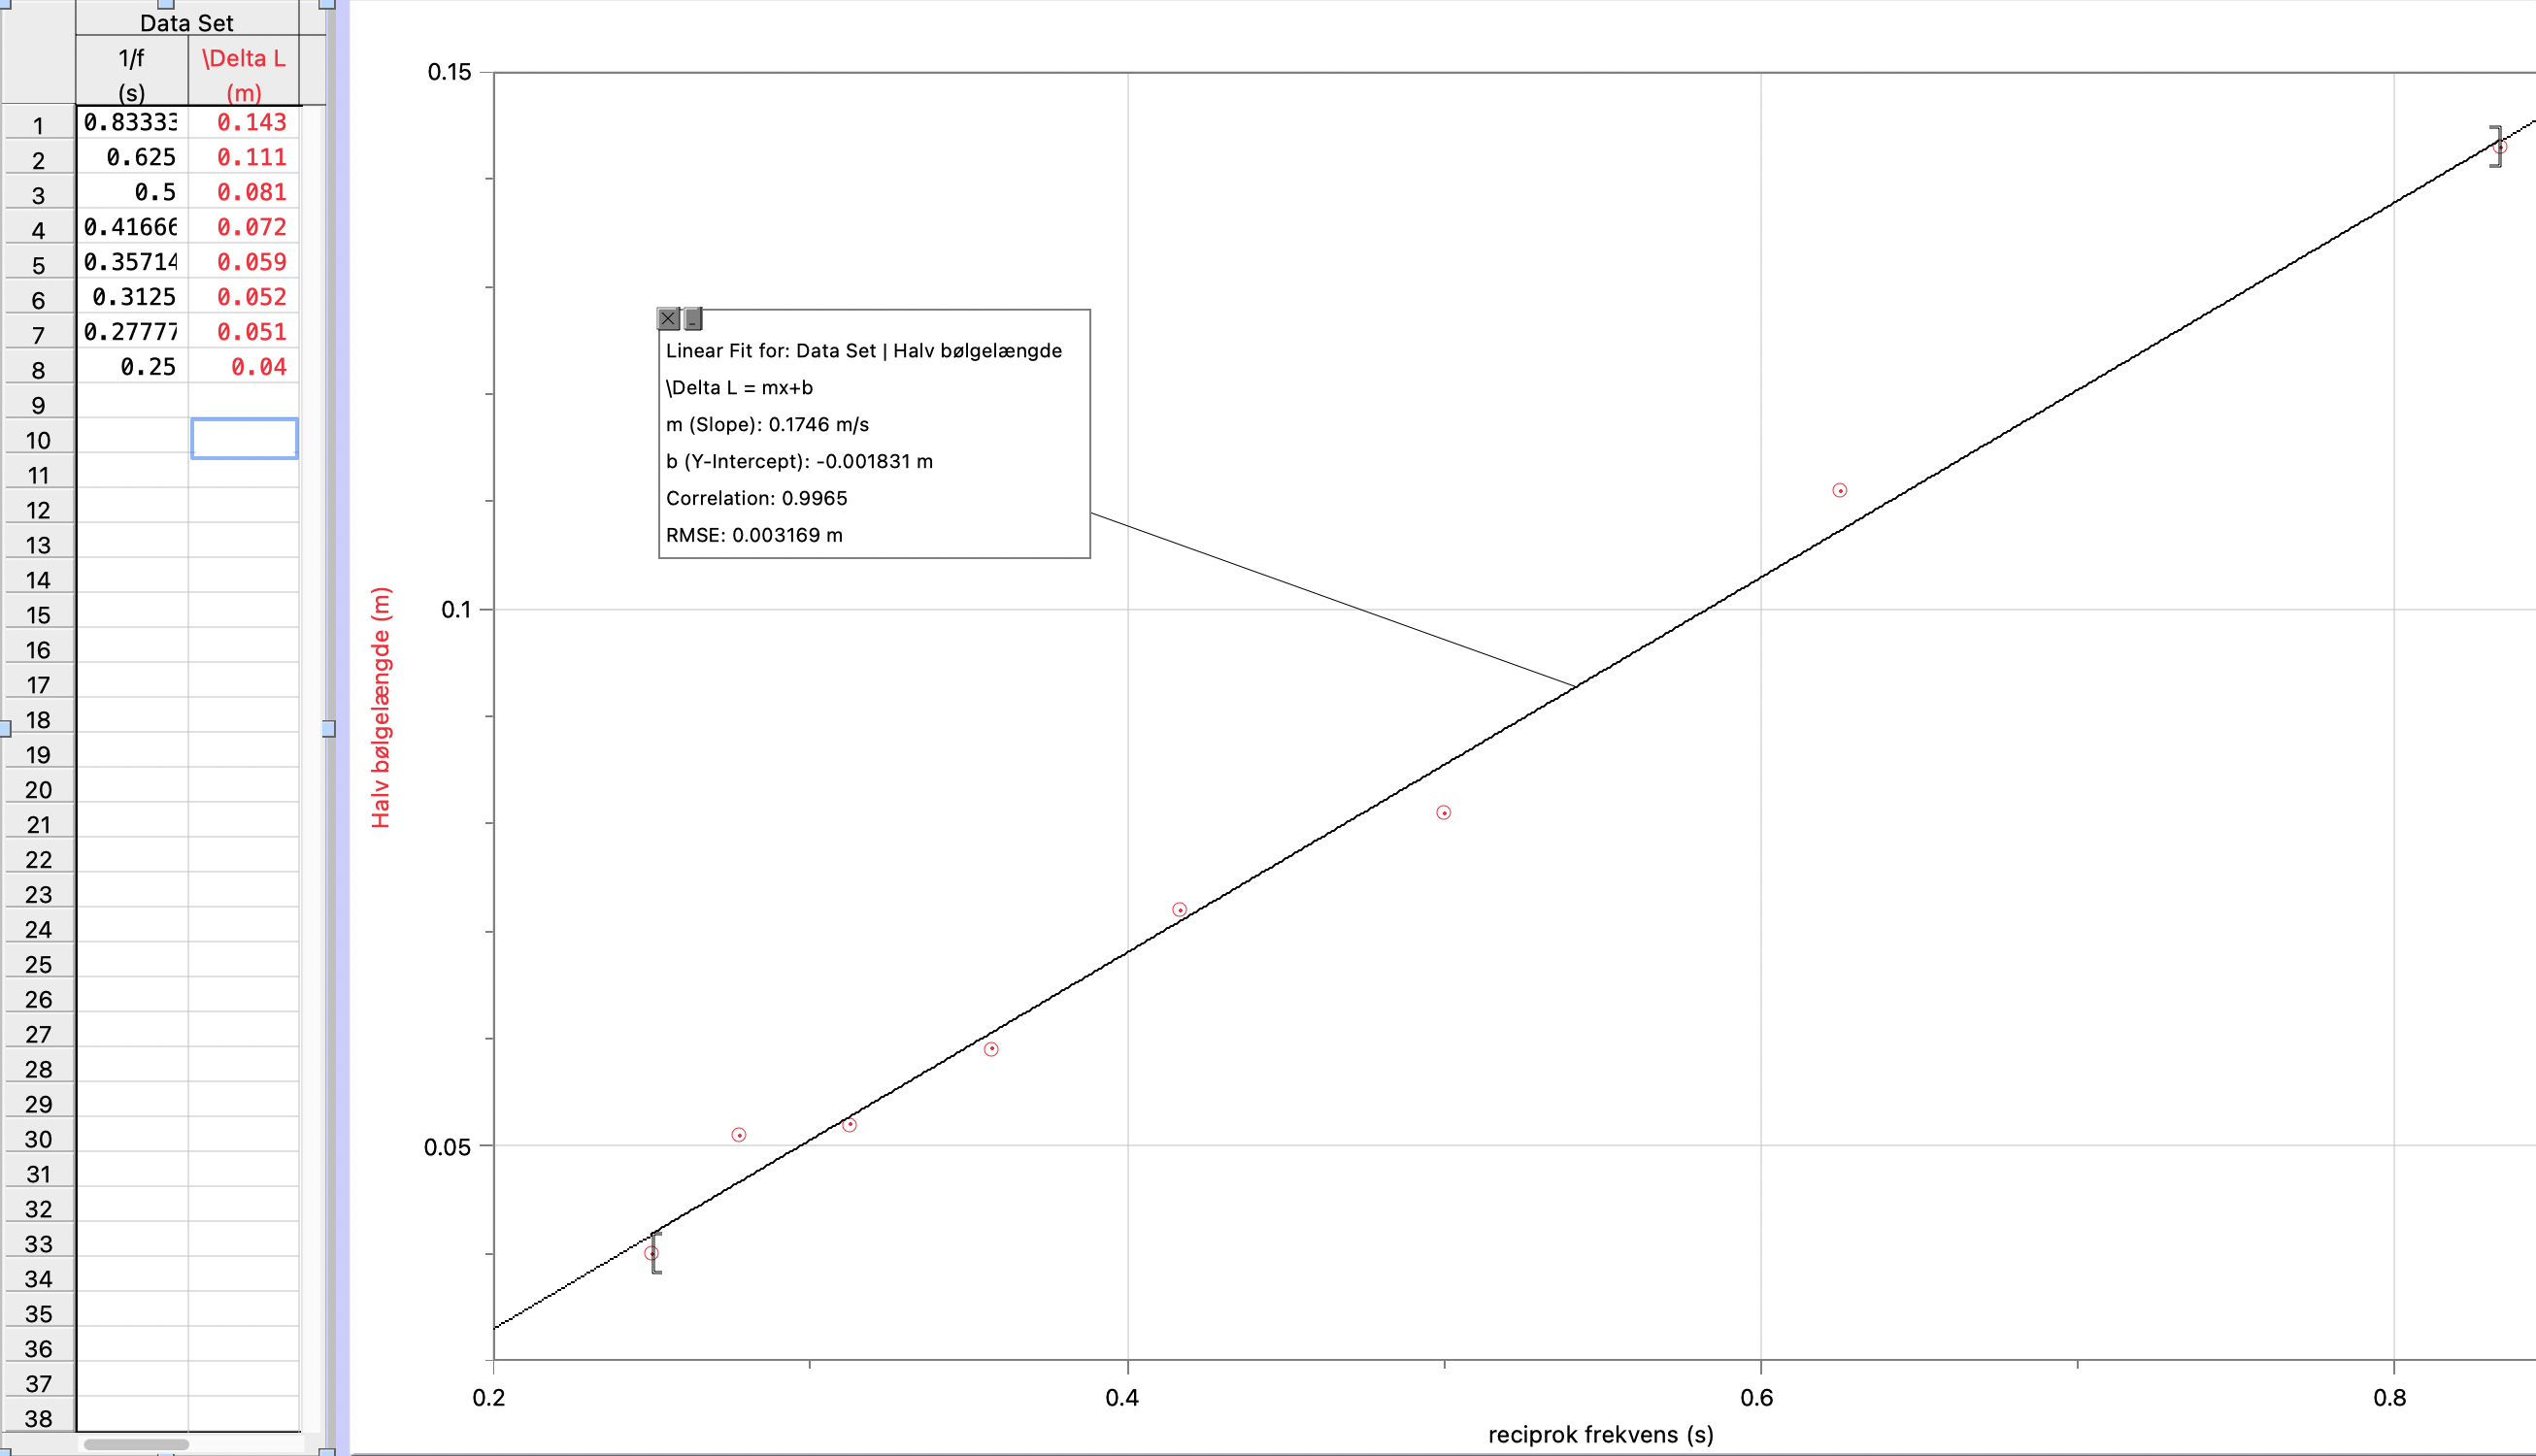
\includegraphics[width=\textwidth]{interferens.png}
\end{center}
\caption{Tabellens data sat ind i Logger Pro}
\label{fig:interferens}
\end{figure}
Siden lydbølgerne har bølgelængden $2 \cdot \Delta L$, må den dobbelte hældning da være lydens fart.
Her denoterer $m$ hældningen. 
\begin{equation*}
\begin{split}
  v&=2 \cdot m \\ 
  &= 2 \cdot 174,6 \;\unit{m/s} \\ 
  &\approx 3,5 \cdot 10^2 \;\unit{m/s} 
\end{split}
\end{equation*}
Altså er lydens fart i luft $3,5 \cdot 10^2 \;\unit{m/s} $.
\section*{Opgave 4}
\sol \\
\textbf{a.}
Den gennemsnitlige acceleration i denne bevægelse er
\begin{equation*}
\begin{split}
  a_{\text{gns} }&= \frac{\Delta v}{\Delta t}\\ 
  &=\frac{3,2 \;\unit{m/s} }{3,1 \cdot 10^{-4} \;\unit{s} }\\ 
  &\approx 1,0 \cdot 10^{4} \;\unit{m/s^2} 
\end{split}
\end{equation*}
Altså er den gennemsnitlige acceleration i denne bevægelse $1,0 \cdot 10^{4} \;\unit{m/s^2} $.\\[1ex]
\textbf{b.}
Da pollenkornet opnår en konstant fart, ser vi på grafens hældning til sidst for at finde farten.
\begin{equation*}
\begin{split}
  v&=\frac{\Delta s}{\Delta t}\\ 
  &=\frac{0,002 \;\unit{m} }{0,02 \;\unit{s} }\\ 
  &=0,1 \;\unit{m/s} 
\end{split}
\end{equation*}
Altså er pollenkornets fart $0,1 \;\unit{m/s} $ når den opnår den konstante fart.\\[1ex]
\textbf{c.}
I starten ser vi, at accelerationen er tilnærmelsesvis konstant og er
\begin{equation*}
\begin{split}
  a&=\frac{\Delta v}{\Delta t}\\ 
  &=\frac{1,0 \;\unit{m/s} }{0,010 \;\unit{s} }\\ 
  &=100 \;\unit{m/s^2} 
\end{split}
\end{equation*}
Fra Newtons 2. lov har vi så, at den samlede kraft nedad må være 
\begin{equation*}
\begin{split}
  F_{\text{res} }&= m \cdot a\\ 
  &= 3,7 \cdot 10^{-12} \;\unit{kg} \cdot 100 \;\unit{m/s^2} \\ 
  &=3,7 \cdot 10^{-10} \;\unit{N} 
\end{split}
\end{equation*}
Størrelsen af luftmodstanden må da være forskellen mellem den samlede kraft og tyngdekraften på pollenkornet.
\begin{equation*}
\begin{split}
  F_{\text{luft} }&= F_{\text{res}} -F_t\\ 
  &=3,7 \cdot 10^{-10} \;\unit{N} -  3,7 \cdot 10^{-12} \;\unit{kg} \cdot 9,82 \;\unit{m/s^2} \\ 
  &\approx 3,3 \cdot 10^{-10} \;\unit{N} 
\end{split}
\end{equation*}
Altså er størrelsen af luftmodstanden på pollenkornet i starten af bevægelsen $3,3 \cdot 10^{-10} \;\unit{N} $.
\section*{Opgave 5}
\sol \\
\textbf{a.}
\ce{^85_36Kr} henfalder ved $\beta^-$ henfald. 
Reaktionsskemaet må da være 
\[
\ce{^85_36Kr -> ^85_37Rb + ^0_{-1}e + \bar{\nu}} 
\] 
Vi ser, at både nukleontal, ladning og leptontal er bevarede: 
\begin{equation*}
\begin{split}
  A&: 85=85+0+0\\ 
  Z&: 36=37-1+0 \\ 
  L&: 0=0+1-1
\end{split}
\end{equation*}
\textbf{b.}
Halveringstiden for \ce{^85_36Kr} er $3,4 \cdot 10^8 \;\unit{s} $.
Vi finder først antallet af kerner ved produktion.
\begin{equation*}
\begin{split}
  N_0&=\frac{A_0}{k}\\ 
  &=\frac{A_0}{\frac{\ln (2)}{T_{1/2}}}\\ 
  &=\frac{2,0 \cdot 10^3 \;\unit{Bq} }{\frac{\ln(2)}{3,4 \cdot 10^8 \;\unit{s} }}\\ 
  &=9,81033 \cdot 10^{11} 
\end{split}
\end{equation*}
Vi ser imidlertid, at
\begin{equation*}
\begin{split}
  1 \;\unit{y} &= 365,25 \cdot 24 \cdot 60^2 \;\unit{s} \\ 
  &=31557600 \;\unit{s} 
\end{split}
\end{equation*}
Vi bruger nu henfaldsloven til at finde antallet af kerner efter 5 år. 
\begin{equation*}
\begin{split}
  N&=N_0 \cdot \left(\frac{1}{2}\right)^{\frac{t}{T_{1/2}}}\\ 
  &= 9,81033 \cdot 10^{11} \cdot \left(\frac{1}{2}\right)^{\frac{5 \cdot 31557600 \;\unit{s} }{3,4 \cdot 10^8 \;\unit{s} }}\\ 
  &=7,11182 \cdot 10^{11}
\end{split}
\end{equation*}
Ved opslag på Ptable ses, at de hver især vejer $84,912527331 \;\unit{u} $.
Altså må den samlede masse være 
\begin{equation*}
\begin{split}
  m&=N \cdot 84,912527331 \;\unit{u} \\ 
  &= 7,11182 \cdot 10^{11} \cdot 84,912527331 \;\unit{u} \cdot 1,661 \cdot 10^{-27} \;\unit{kg/u} \\ 
  &\approx 1,0 \cdot 10^{-13} \;\unit{kg} 
\end{split}
\end{equation*}
Altså er massen af \ce{^85_36Kr} efter 5 år $1,0 \cdot 10^{-13} \;\unit{kg} $.
\section*{Opgave 6}
\sol \\
\textbf{a.}
Siden brydningsindekset angiver, hvor mange gange lyset fart i vakuum er større end i det pågældende stof, så må lysets fart inde i krystallen være 
\begin{equation*}
\begin{split}
  v&=\frac{c}{n}\\ 
  &=\frac{2,9979 \cdot 10^8 \;\unit{m/s} }{1,470}\\ 
  &\approx 2,039 \cdot 10^8 \;\unit{m/s} 
\end{split}
\end{equation*}
Altså er lysets fart inde i krystallen $2,039 \cdot 10^8 \;\unit{m/s} $.\\[1ex]
\textbf{b.}
Hver \ce{Nd^3+}-ion har energien 
\begin{equation*}
\begin{split}
E_{\text{ion} }&=0,201 \cdot 10^{-18} \;\unit{J} -0,012 \cdot 10^{-18} \;\unit{J} \\ 
  &=0,189 \cdot 10^{-18}\;\unit{J} 
\end{split}
\end{equation*}
Vi kan nu beregne antallet af ioner der hopper energiniveau hvert sekund.
\begin{equation*}
\begin{split}
  N&=\frac{P \cdot \Delta t}{E_{\text{ion} }}\\ 
  &=\frac{0,50 \;\unit{W} \cdot 1 \;\unit{s} }{0,189 \cdot 10^{-18}\;\unit{J} }\\ 
  &\approx 2,6 \cdot 10^{18} 
\end{split}
\end{equation*}
Altså overgår $2,6 \cdot 10^{18}$ \ce{Nd^3+}-ioner hvert sekund fra energiniveau B til energiniveau A.
\end{document}
